\documentclass[handout]{beamer}

\newcommand{\darkLogo}{$\vcenter{
\includegraphics{tallogo-dark.pdf}}$}
\usepackage{wrapfig}
\usefonttheme{serif}
\usepackage[no-math]{fontspec}
\usepackage{ amsmath
           , amsfonts
           , amssymb
           , stmaryrd
           , fontawesome
           , epigraph
           }

\def\lnk#1{\href{#1}{\faFilePdfO}}

\def\yo{\text{y}}
\def\pto{\rightsquigarrow}
\def\Prof{\textbf{Prof}}
\def\Lan{\text{Lan}}

\definecolor{bleakYellow}{HTML}{F0DB4F}
\setmainfont{Source Sans Pro}

\usetheme[background=dark]{metropolis}
\setbeamercolor{alerted text}{fg=bleakYellow}

\setbeamertemplate{footline}{}

\title{Fosco Loregian \darkLogo}
\author{}
\date{May 19 2020}

\setbeamertemplate{navigation symbols}{}

\hypersetup{colorlinks,linkcolor=,urlcolor=green}

\usetikzlibrary{
    cd, % to make easy commutative diagrams
    petri, % To draw petri nets
    backgrounds, % To define image backgrounds
    arrows, % To use and define further arrow tips
    positioning, % To use expressions like "right = 1 of 1"
    decorations.markings, % Needed to define oriented wiring diagrams
    calc,  % Needed to define oriented wiring diagrams
    fit, % Needed to compose wiring diagrams
    shapes.multipart
  }

\tikzstyle{place}=
[circle,thick,draw=blue!75,fill=blue!20,minimum size=6mm]
\tikzstyle{antiplace}=
[circle,thick,draw=red!75,fill=red!20,minimum size=6mm]
\tikzstyle{transition}=
[rectangle,thick,draw=black!75,fill=black!20,minimum size=4mm]
\tikzstyle{inarrow}=[->, >=stealth, shorten >=.03cm,line width=1.5]
\tikzstyle{antiarrow}=[<-, red!75,  >=stealth, shorten >=.03cm,line width=1.5]


\tikzset{
	pics/netA/.style args={#1/#2/#3/#4/#5/#6/#7}{code={
					% \fill[yellow!15] (-0.8,-2.3) rectangle (2.3, 2.3);

					\node [place,label=above:$p_1$, tokens={%
								#1
							}] (-pl_1) {};

					\node [transition,label=above:$t$, label=below:#5] (-tr_1) [right = of -pl_1] {};

					\node [place,label=above:$p_2$, tokens={%
								#2
							}] (-pl_2) [right = of -tr_1] {};

					\node [transition,label=left:$v$, label=above:#6] (-tr_2) [below = of -tr_1] {};
					\node [transition,label=below:$u$, label=above:#7] (-tr_3) [below = of -tr_2] {};

					\node [place,label=below:$p_3$, tokens={%
								#3
							}] (-pl_3) [left = of -tr_3] {};

					\node [place,label=below:$p_4$, tokens={%
								#4
							}] (-pl_4) [right = of -tr_3] {};

					\draw[inarrow] (-pl_1) -- (-tr_1);
					\draw[inarrow] (-tr_1) -- (-pl_2);
					\draw[inarrow] (-pl_2) -- (-tr_2);
					\draw[inarrow] (-tr_2) -- (-pl_3);
					\draw[inarrow] (-tr_2) -- (-pl_4);
					\draw[inarrow] (-pl_3) -- (-tr_3);
					\draw[inarrow] (-tr_3) -- (-pl_4);
				}}
}

\begin{document}
\begin{frame}
  \maketitle
\end{frame}
\begin{frame}{Past \& present positions}
  \begin{itemize}
    \item<+-> Ph.D. at SISSA - Trieste IT 
\includegraphics{ita.pdf} (but advisor in Rome, {\color{magenta} D. Fiorenza})

    \indent {\footnotesize\color{gray!40} Stable homotopy theory, ∞-categories, derived AG}
    \item<+-> University of Western Ontario - London CA 
\includegraphics[scale=.04]{can.pdf}

    \indent {\footnotesize\color{gray!40} ∞-categories, derivators}
    \item<+-> Masaryk University - Brno CZ 
\includegraphics{czr.pdf}

    \indent {\footnotesize\color{gray!40} Accessible categories, derivators, 2-categories}
    \item<+-> Max Planck Inst. für Math. - Bonn D 
\includegraphics{ger.pdf}

    \indent {\footnotesize\color{gray!40} 2-categories, derivators, applied category theory}
    \item<+-> Centro de Matemàtica - Coimbra PT 
\includegraphics[scale=.04]{por.pdf}

    \indent {\footnotesize\color{gray!40} 2-categories; finishing my first book}
    \item<+-> Tallinna Tehnikaülikooli - Tallinn EE 
\includegraphics{est.pdf}

    \indent {\footnotesize\color{gray!40} 2-categories; functorial semantics; categorical probability theory and its applications}
  \end{itemize}
\end{frame}
%
%
%
%
%
\begin{frame}
  \Huge\centering \bfseries STABLE HOMOTOPY THEORY
\end{frame}
%
\begin{frame}
  \alert{∞-categories}: a thickening of the notion of category, suitable for homotopy-coherent mathematics (math.AG, math.AT, math.LO, cs.PL\dots).

  \onslide<2->
  % Turns out some parts of Mathematics are easier if stated in these terms:
  % \begin{itemize}
  %   \item<+-> {\footnotesize \color{gray!60} homological algebra : the scary part of algebraic topology}

  %   \lnk{www.blank.com}{\color{green} higher algebra}: the linear algebra of ∞-categories
  %   \item<+-> {\footnotesize \color{gray!60} 1-topos theory : a synthetic type theory}

  %   \lnk{www.blank.com}{\color{green} ∞-topos theory}: a synthetic homotopy theory of homotopy types
  % \end{itemize}
\end{frame}
%
%
%
%
%
\begin{frame}
  A \alert{stable ∞-category} is an ∞-category
\begin{itemize}
\item with all \alert{finite limits and colimits}
\item such that a square is \alert{cartesian iff cocartesian}
\end{itemize}
\begin{itemize}
\item<+-> The homotopy category of a stable ∞-cat is always triangulated.
\item<+-> Sending an abelian category $\cal A$ into its derived category has a nice and clear \alert{universal property} stated in terms of the heart of a canonical $t$-structure.
\item<+-> Stable, rational, $p$-adic, ...  homotopy theory become pieces of the commutative algebra of  ∞-categories.
\end{itemize}
\end{frame}
%
%
%
%
%
\begin{frame}{Each PhD starts with a question}
  A \alert{t-structure} on a triangulated $\cal D$ is a pair of triangulated subcategories of $\cal D$ such that every object X lies in a sequence
\[X_{\le} \to X \to X_\ge \to X_\le[1]\]
[\alert{FL14} \lnk{https://link.springer.com/article/10.1007/s10485-015-9393-z}] : On stable ∞-categories a t-structure is a factorization system $(E,M)$
\begin{itemize}
\item<+-> such that $E$ and $M$ are 3-for-2 classes
\item<+-> thus the category of $E$-cofibrant objects is coreflective
\item<+-> and the category of $M$-fibrant objects is reflective
\item<+-> cof/fib replacement = $\pm$ truncation
\end{itemize}
\end{frame}
%
%
%
\begin{frame}{Plan: redo $t$-structures (w/ Domenico)}
  \begin{itemize}
\item<+-> {} [\alert{FLM15} \lnk{https://link.springer.com/article/10.1007/s40062-019-00237-0}] The set of t-structures has a natural choice of $\mathbb Z$-action ($\mathbb Z$ = the integers); so, study $\mathbb Z$-equivariant monotone maps from a poset $P$ to $TS(\cal C)$. These are called \alert{slicings}

{\footnotesize\color{gray!40} apply to: describe Bridgeland stability manifolds [\alert{L-PhD\lnk{http://tetrapharmakon.github.io/stuff/main.pdf}}], and Postnikov towers on ∞-toposes.}

\item<+-> {} [\alert{FL15b} \lnk{https://arxiv.org/abs/1507.03913}] Every stratified manifold $(X,\mathfrak s)$ generates a pair of t-structure that can be glued together

{\footnotesize\color{gray!40} apply to: recollements, stratified schemes, representation of algebras}

  \end{itemize}
\end{frame}
%
%
%
%
%
\begin{frame}{Plan: redo $t$-structures (w/ Domenico)}\small
   \begin{itemize}
     \item<+-> The set of \alert{slicings} on a stable ∞-category has a metrizable topology

     \item<+-> The space \[\{ J \colon \mathbb R \to TS(\mathcal C) \mid J \text{ is Sorgenfrey continuous} \}\]
     is an interesting set [\alert{L-PhD}\lnk{http://tetrapharmakon.github.io/stuff/main.pdf}]. Bridgeland: demistified.
    \end{itemize}

    \onslide<+->
    \begin{block}{Conjecture}
\vspace{.5mm}
  Study
\[\{ J \colon \text{Spec}(\mathbb Z) \to TS(\mathcal D(X_p)) \mid J \text{ is Zariski continuous} \}\]
($X_p$ a variety in positive characteristic) to get something about motivic t-structure.
 \end{block}
 \onslide<+->
 \begin{block}{Conjecture}
\vspace{.5mm}
 Blakers-Massey in positive characteristic is a theorem about factorization systems.
 \end{block}
\end{frame}
%
%
%
%
\begin{frame}{Todo: Morse theory is a theory of FS}
  \begin{wrapfigure}[5]{l}{.5\textwidth}
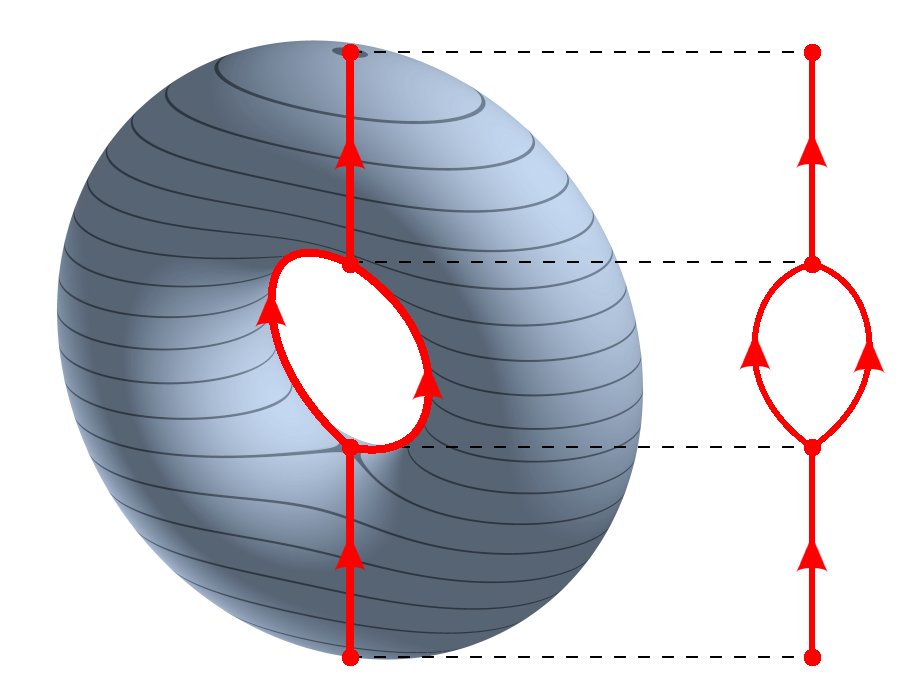
\includegraphics[scale=.15]{3D-Leveltorus-Reebgraph.png}
  \end{wrapfigure}

  % \onslide<2->
  $\textbf{Bord}(n)$ is the free (∞,\emph{n})-symmoncat on the point.

  \vspace{1cm}
  \onslide<2->Tensor~functors $Z : Bord(n) \to Vect$ are completely classified.

  \vspace{1cm}
  \onslide<3->
  Morse theory is the theory of suitable factorization systems on Bord(n).

  \alert{critical points of a Morse function}
  correspond to

 \alert{critical values} [\alert{L-PhD}, Ch.7] of a certain slicing $J : \mathbb R \to FS(Bord(n))$.
\end{frame}
%
%
%
%
%
%
%
\begin{frame}
  \Huge\centering \bfseries DERIVATORS
\end{frame}
%
\begin{frame}{The formal category theory of derivators}
  A \alert{derivator} is a strict 2-functor
  \[\mathbb{D} : {\bf Cat}^\text{op} \to {\bf CAT} \]
  satisfying stacky conditions. They form the 2-category \textbf{Der}.

  They subsume most of ∞-category theory; in particular, their stable homotopy.
  \begin{itemize}
    \item<2-> [{[\alert{LV17}\lnk{https://www.sciencedirect.com/science/article/abs/pii/S0021869320300296}]}] : A t-structure on a stable derivator is still a certain kind of factorization system;

    {\footnotesize\color{gray!40} FS are still \alert{strict 2-algebras} for the "squaring" 2-monad ( \_ )²}% : $\mathcal A \mapsto \mathcal A^2$ (see [\emph{KT93}])}

    \item<3->  [{[\alert{Lor18}\lnk{https://arxiv.org/abs/1802.08193}]}] : reflective subderivators correspond to reflective factorization systems, and to algebras for idempotent monads

    {\footnotesize\color{gray!40} (the \alert{formal theory of monads} [\emph{S80}] still holds in \textbf{Der})}%, a monad $T : D \to D$ is just defined objectwise)}
  \end{itemize}
\end{frame}
%
\begin{frame}{The formal category theory of derivators}
  There is a \alert{Yoneda structure}\footnote{A 2-categorical device to encode the calculus of pointwise Kan extensions.} on the 2-category of derivators
\begin{itemize}
\item<2-> notions of \alert{accessible} and \alert{locally presentable} derivator using the theory of LPAO in a Yoneda structure, done in [\alert{DLL18}\lnk{https://arxiv.org/abs/1804.08710}];

{\footnotesize\color{gray!60} categorical logic for derivators (see Prest's treatment of \alert{definability} for module categories); derivator \alert{topos theory}?}
\item<3-> \alert{adjoint functor theorem}s for derivators;

{\footnotesize\color{gray!60} existence of a \alert{six-operation} calculus. 2-categorical account of Grothendieck duality complicated diagrams (without multicategories)}
\item<4-> \alert{profunctors} between derivators; fibered derivators;

{\footnotesize\color{gray!60} \alert{operads} in derivator theory; applications in representation theory of algebras, stable homotopy, ...}
\end{itemize}
\end{frame}
%
%
%
%
%
%
\begin{frame}
  \Huge\centering \bfseries COEND CALCULUS% AND DG-STUFF
\end{frame}
%
\begin{frame}{Coends}
  I have written a book [\alert{L20}\lnk{https://arxiv.org/pdf/1501.02503}] on \alert{coend calculus}, soon to appear under Cambridge LNSs:
\begin{wrapfigure}{l}{.35\textwidth}
  
\includegraphics[width=.35\textwidth]{cover-2-.pdf}
\end{wrapfigure}
\small
\begin{itemize}
  \item<+-> Coends $\int_C T$ are universal objects associated to $T : C^{op}\times C \to D$, treated as integrals (a ``Fubini rule'' is valid).
  \item<+-> applications in (monoidal) category theory, algebraic topology, universal algebra, algebraic geometry, categorical logic, representation theory (see ch.7 for an application to \alert{DG-categories}), functional programming\dots
  \item<+-> The book is being extensively cited (45 citations on Scholar \today)
\end{itemize}
\end{frame}
%
%
%
%
\begin{frame}{DG-stuff}
  Coends are useful for
\begin{itemize}
  \item category theory
  \item functional programming
  \item algebraic geometry
  \item algebraic topology
  \item module/representation theory
  \item \dots
\end{itemize}
A book about them needed to be written.
\end{frame}

\begin{frame}
  \Huge\centering \bfseries CATEGORICAL SEMANTICS OF NETS
\end{frame}
\begin{frame}
A Petri net is a certain mathematical model for distributed systems.

A Petri net is a presentation for a free (commutative) monoidal category.
\begin{center}
  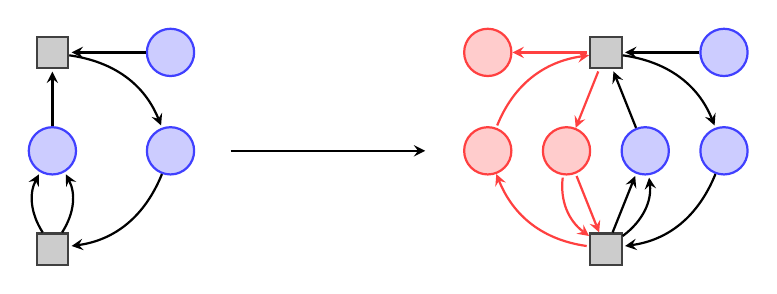
\begin{tikzpicture}
		\begin{scope}[xshift=-100]
			% \begin{pgfonlayer}{nodelayer}
				\node [place,tokens=0] (1a) at (1.5,1.25) {};
				\node [place,tokens=0] (1b) at (-0,0) {};
				\node [place,tokens=0] (3a) at (1.5,0) {};
				\node[transition] (2a) at (0,1.25) {};
				\node[transition] (2b) at (0,-1.25) {};
			% \end{pgfonlayer}
			% \begin{pgfonlayer}{edgelayer}
				\draw[style=inarrow, thick] (1a) to (2a);
				\draw[style=inarrow, thick] (1b) to (2a);
				\draw[style=inarrow, thick, bend right] (2b) to (1b);
				\draw[style=inarrow, thick, bend left] (2b) to (1b);

				\draw[style=inarrow, thick, bend left] (2a) to (3a);
				\draw[style=inarrow, thick, bend left] (3a) to (2b);
			% \end{pgfonlayer}
		\end{scope}

		\begin{scope}[xshift=100]
			% \begin{pgfonlayer}{nodelayer}
				\node [place,tokens=0] (1a) at (1.5,1.25) {};
				\node [place,tokens=0] (1b) at (0.5,0) {};
				\node [place,tokens=0] (3a) at (1.5,0) {};
				\node [antiplace,tokens=0] (1ax) at (-1.5,1.25) {};
				\node [antiplace,tokens=0] (1bx) at (-0.5,0) {};
				\node [antiplace,tokens=0] (3ax) at (-1.5,0) {};
				\node[transition] (2a) at (0,1.25) {};
				\node[transition] (2b) at (0,-1.25) {};
			% \end{pgfonlayer}
			% \begin{pgfonlayer}{edgelayer}
				\draw[style=inarrow, thick] (1a) to (2a);
				\draw[style=inarrow, thick] (1b) to (2a);
				\draw[style=inarrow, thick, bend right] (2b) to (1b);
				\draw[style=inarrow, thick] (2b) to (1b);

				\draw[style=inarrow, thick, bend left] (2a) to (3a);
				\draw[style=inarrow, thick, bend left] (3a) to (2b);

				\draw[style=antiarrow, thick] (1ax) to (2a);
				\draw[style=antiarrow, thick] (1bx) to (2a);
				\draw[style=antiarrow, thick] (2b) to (1bx);
				\draw[style=antiarrow, thick, bend left] (2b) to (1bx);

				\draw[style=antiarrow, thick, bend right] (2a) to (3ax);
				\draw[style=antiarrow, thick, bend right] (3ax) to (2b);
			% \end{pgfonlayer}
		\end{scope}


		\draw[style=inarrow, thick] (-1.25,0) -- (1.25,0);
	\end{tikzpicture}
\end{center}
\begin{center}
  Study monoidal categories: you will understand Petri nets.
\end{center}
\end{frame}
\begin{frame}
Extensions of Petri nets:
\begin{itemize}
  \item Genovese, Fabrizio, Fosco Loregian, and Daniele Palombi.
  \alert{A Categorical Semantics for Bounded Petri Nets.}
   \href{https://arxiv.org/pdf/2101.09100}{arXiv:2101.09100} (2021), ACT2021.
  \item Genovese, Fabrizio, and Jelle Herold.
  \alert{A Categorical Semantics for Hierarchical Petri Nets.}
   \href{https://arxiv.org/pdf/2102.00096}{arXiv:2102.00096} (2021), GCM2021.
  \item Genovese, Fabrizio, Fosco Loregian, and Daniele Palombi.
  \alert{Nets with Mana: A Framework for Chemical Reaction Modelling.}
   ICGT 2021.
\end{itemize}
\end{frame}
%
%
%
%
%
\begin{frame}
  \Huge\centering \bfseries TEACHING AND ORGANIZATIONAL ACTIVITIES
\end{frame}
%
\begin{frame}{Teaching and\dots}\small
  \begin{itemize}
    \item<+-> 2015 A short course on \alert{model categories} {\color{magenta} @unipv};
    \item<+-> 2016 ``\alert{Elements of Finite Mathematics}'' {\color{magenta} @uwo} (mostly statistics to kinesiologists).
    \item<+-> 2016 \alert{Advisor} of a BSc thesis {\color{magenta} @unibo}, "Elementary aspects of adjoint functors". I enjoyed it!
    \item<+-> 2018 A short course on \alert{2-category theory} {\color{magenta} @unipd}: monoidal and enriched, categories, the calculus of coends and Kan extensions, bicategories, monads...
    \item<+-> 2020 \alert{Category theory} course Teacher {\color{magenta} @taltech}. Mentoring activity for MSc students interested in category theory in CS.
\end{itemize}
\end{frame}
\begin{frame}{Teaching and\dots}\small
  \begin{itemize}
    \item<+-> advisor for master student's thesis: \emph{M. Roselli}, `Categorical linguistics'
    \item<+-> advisor for master student's thesis: T. Massacrier, `Differential Polynomial endofunctors'

    {\footnotesize\color{gray!40} based on arXiv:2103.00938\lnk{https://arxiv.org/abs/2103.00938}}
    \item<+-> SIGPLAN's mentor: long-term mentoring program for programming languages researchers.

    {\footnotesize\color{gray!40} frequent PRs to the \href{https://github.com/agda/agda-categories}{agda-categories} library}

\end{itemize}
\end{frame}
\begin{frame}{Organisation of conferences}\small
  \begin{itemize}
    \item<+-> 2015 and 2019 Attendee and speaker at the \alert{Kan Seminar I}

    {\footnotesize\color{gray!40} a webinar on category theory}
    \item<+-> and \alert{Applied Category Theory} 2019

    {\footnotesize\color{gray!40} (a webinar on applied category theory, from which the paper [\alert{MLR$^{+}$20}\lnk{https://arxiv.org/abs/2001.07488}] stemmed)}
    \item<+-> 2018 \alert{Organiser} of the 103rd \alert{PSSL}

    {\footnotesize\color{gray!40} Peripathetic Seminar on Sheaves and Logic, Brno.}
    \item<+-> 2019 and 2020 Among the \alert{organisers} of ItaCa

    {\footnotesize\color{gray!40}  \alert{Ita}lian \alert{Ca}tegory theorists) in Milan and soon on zoom, due to COVID19.}
    \item<+-> Reviewer for zbMath and AMS.
  \end{itemize}
\end{frame}
%
%
%
%
%
%
%
\begin{frame}{Miscellaneous projects}
\small
\begin{itemize}
  \item<+-> Homotopy theory and set theory: [\alert{DL18}\lnk{https://link.springer.com/article/10.1007/s40062-018-0197-3}]

  {\color{gray!70}\footnotesize  no homotopy category of a model category is ``concrete''; what about ∞-categories?}
  \item<+-> Functional programming and type theory:

  {\color{gray!70}\footnotesize  HoTT, linear types, proof-checkers, categorical algebra in relational database architecture; natural language processing using category theory\dots}
  \item<+-> Categorical logic and foundations of mathematics;

  {\color{gray!70}\footnotesize  functorial semantics \emph{à la} Lawvere, but sprinkled with operads and multicategories.}
  \item<+-> more in detail, ``2-semantics'' of algebraic theories:

  {\color{gray!70}\footnotesize profunctorial PROPs and theories, categorical algebra of cartesian bicategories\dots}
\end{itemize}
\end{frame}
%
\begin{frame}
% \begin{itemize}
Reach me out at \href{http://tetrapharmakon.github.io}{my web page}:
\begin{center}
\href{http://tetrapharmakon.github.io}{
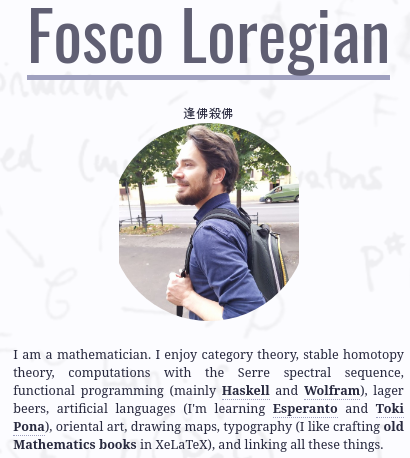
\includegraphics[width=.2\textwidth]{crop1.png}
}
\end{center}
% \item I'm quite open about my projects:
% \begin{center}
%   \href{https://github.com/tetrapharmakon}{\faGithub \kern1em tetrapharmakon}
% \end{center}
% \item Taltech has an extremely active \href{https://compose.ioc.ee}{ongoing CT seminar}:
% \begin{center}
% \href{https://compose.ioc.ee}{
% 
\includegraphics[width=.3\textwidth]{crop2.png}
% }
% \end{center}
% Reach us out!
% \end{itemize}
% \setlength{\epigraphwidth}{.75\textwidth}
% \epigraph{\footnotesize A human being should be able to change a diaper, plan an invasion, butcher a hog, conn a ship, design a building, write a sonnet, balance accounts, build a wall, set a bone, comfort the dying, take orders, give orders, cooperate, act alone, solve equations, analyze a new problem, pitch manure, program a computer, cook a tasty meal, fight efficiently, die gallantly. Specialization is for insects.}{R. Heinlein}
\end{frame}
%
%
%
%
%
\end{document}
